\documentclass{article}
\usepackage[utf8]{inputenc}
\usepackage{amsmath, amssymb}
\usepackage{graphicx}
\usepackage{wrapfig}
\graphicspath{ {./images/} }




\newcommand\tab[1][1cm]{\hspace*{#1}}
\newcommand{\newVec}[2]{\begin{bmatrix}#1 \\ #2 \end{bmatrix}}
\newcommand{\newVect}[3]{\begin{bmatrix}#1 \\ #2 \\ #3\end{bmatrix}}
\newcommand{\newtt}[4]{\begin{bmatrix}#1 & #2\\ #3 & #4 \end{bmatrix}}
\newcommand{\newttt}[9]{\begin{bmatrix}#1 & #2 & #3\\ #4 & #5 & #6 \\ #7 & #8 & #9\end{bmatrix}}


\title{Linear Algebra Homework 4}
\author{William Jardee}
\date{March 2020}

\begin{document}

\maketitle

\begin{enumerate}
    \item 
\tab Prove Theorem 4.21(c)"\par
"If $A \sim B$ and $B \sim C$, then $A \sim C$"\\\\
Proof:\par
Let A, B, and C be $n \times n$ matrices. If $A \sim B$ and $B \sim C$, then by definition of similar matrices: $A = P^{-1} B P$ and $B = Q^{-1} C Q$.By substitution: $A = P^{-1}Q^{-1}CPQ$. It is evident that $(P^{-1}Q^{-1})(PQ) = I$, so $(P^{-1}Q^{-1})$ and $(PQ)$ are inverses. Renaming $PQ$ as $S$, $A = S^{-1}CS$. By definition of similar matrices, $A \sim C$.\par
{\raggedleft "Quack"  $\blacksquare$\\}

\item
\tab Prove Theorem 4.22(b)\par
"Let A and B be $n \times n$ matrices with $A \sim B$, then A is invertible if and only if B is invertible."\\\\
Proof:\par
Let A and B be $n \times n$ matrices such that $A \sim B$. By definition of similar matrices, $A = P^{-1}BP$. If we assume A is invertible, it follows that\\
\tab $A^{-1} = (P^{-1}BP)^{-1} = PB^{-1}P^{-1}$\\
So in order for A to be invertible, then B must be invertible. The equality proves if and only if relationship.\par
{\raggedleft "Quack"  $\blacksquare$\\}

\item
\tab Prove Theorem 4.22(f)\par
"Let A and B be $n \times n$ matrices with $A \sim B$, then $A^{m} \sim B^{m}$ for all integers $m \geq 0$."\\\\
Proof:\par
Let A and B be $n \times n$ matrices such that $A \sim B$. This is be a proof by induction. Let us first establish our base case.\par
Base Case: By definition of similar matrices, $A = P^{-1}BP$. Then $A^2 = AA = P^{-1}BPP^{-1}BP = P^{-1}BBP = P^{-1}B^2P$. So $A^2 \sim B^2$. The case holds for $m = 2$. \par
Inductive Step: Let us assume that $A^k \sim B^k$ for some integer $k \geq 2$. Then $A^{k+1} = AA^{k} = P^{-1}BPP^{-1}B^kP = P^{-1}BB^kP = P^{-1}B^{k+1}P$. So if $A^k \sim B^k$, then $A^{k+1} \sim B^{k+1}$ for all $ k \geq 2$.\par
To account for $m = 1$, this is our original assumption, so this must be true. For any $n \times n$ matrix $Q$, $Q^0 = I$, so $A^0 = I = P^{-1}P = P^{-1}IP = P^{-1}B^0P$. So $A^0 \sim B^0$. The statement can then be generalized to $A^m \sim B^m$ for all integers $m \geq 0$.\par
{\raggedleft "Quack"  $\blacksquare$\\}

\item
Let A and B be $n \times n$ matrices, each with $n$ distinct eigenvalues. Prove that A and B have the same eigenvectors if and only if $AB = BA$.\\\\
Proof:\par
Let A and B be two $n \times n$ matrices with $n$ distinct eigenvalues. We know that A and B are diagonalizable since their are the same number of eigenvalues as the number of dimensions. So, $A = P^{-1} \Lambda P$ and $B = Q^{-1} \Lambda Q$. So $AB = P^{-1} \Lambda PQ^{-1} \Lambda Q$. If $P = Q$, that is to say they have the same eigenvectors, then $AB = Q^{-1} \Lambda QP^{-1} \Lambda P = BA$. If instead of assuming $P = Q$, we assume $AB = BA$, then the following holds. $AB = P^{-1}\Lambda PQ^{-1} \Lambda Q = BA = Q^{-1}\Lambda QP^{-1}\Lambda P$. We see that this is equivalent to substituting P in for Q, and Q for P, so $P = Q$. Both directions hold, so an if and only if relationship exists between the two vectors being diagonalizable and their eigenvectors being equal.\par
{\raggedleft "Quack"  $\blacksquare$\\}

\item
\tab $x' = -0.8x +0.4y$\\ 
\tab $y' = 0.4x -0.2y$\\\\
$  \newVec{x'}{y'} = \newtt{-0.8}{0.4}{0.4}{-0.2} \newVec{x}{y}$\\
$\lambda \newVec{x}{y} = \newtt{-0.8}{0.4}{0.4}{-0.2} \newVec{x}{y}$\\\\
Char Eq:\\ $(-0.8 - \lambda)(-0.2 - \lambda) - (0.4)(0.4) = 0$\\
$(0.16 + \lambda + \lambda^2) - 0.16 = 0$\\
$\lambda^2 + \lambda = 0 = \lambda(\lambda + 1)$\\
$\lambda = 0, \tab \lambda = -1$\\
$\lambda = 0: -0.8x +0.4y = 0 \rightarrow \newVec{1}{2}$\\
$\lambda = -1: -x = -0.8x +0.4y \rightarrow \newVec{1}{-2}$\\
General Solution: $\newVec{x}{y} = C_1e^{0t}\newVec{1}{2} + C_2e^{-t}\newVec{1}{-2}$\par
Since we are asking about activity at $\infty$, we can disregard the $e^{0t}$ term. Instead we can just focus on the solution with respect to that other eigenvector.\par
Plugging in the initial condition of $\newVec{10}{15}$: $C_2 = \frac{35}{4}$, so the solution as we approach infinity looks like: $\frac{35}{4} \newVec{1}{2}$, or just the line $\newVec{1}{2}t$. \\

\item
$A = \newtt{0.5}{-0.5}{0}{0.5}$
\begin{enumerate}
    \item {$\textbf{x}_0 = \newVec{1}{1}\\ \textbf{x}_1 = \newVec{0}{0.5}\\ \textbf{x}_2 = \newVec{-0.125}{0.125}\\ \textbf{x}_3 = \newVec{0}{0.125}$\\
        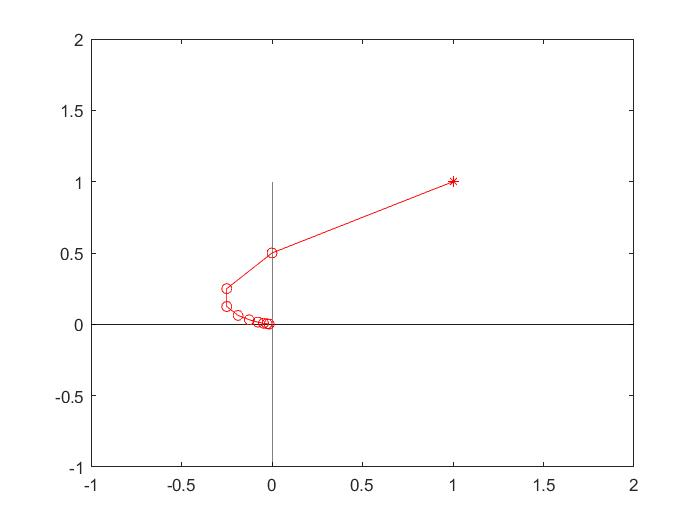
\includegraphics[width=50mm,scale=1]{Matlab1.jpg}
    }
    \item $\textbf{x}_0 = \newVec{1}{0}\\ \textbf{x}_1 = \newVec{0.5}{0}\\ \textbf{x}_2 = \newVec{0.25}{0}\\ \textbf{x}_3 = \newVec{0.125}{0}$\\
    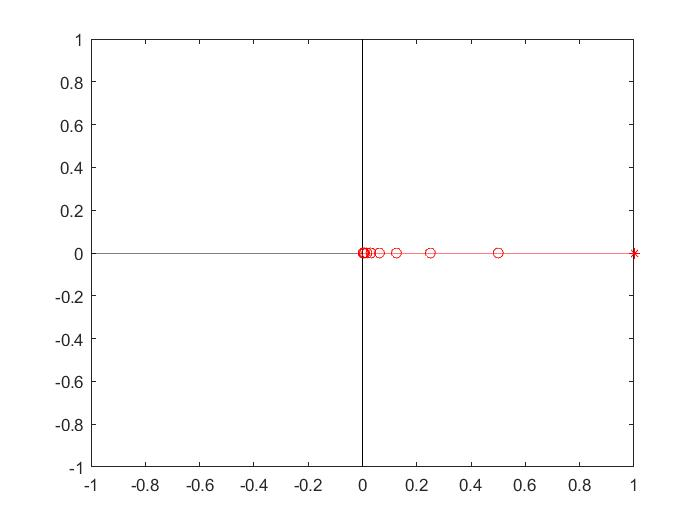
\includegraphics[width=50mm,scale=1]{Matlab2.jpg}

    \item $\lambda \newVec{x}{y} = \newtt{0.5}{-0.5}{0}{0.5}$\\\\
    $(0.5 - \lambda)^2 = 0$\\
    $\lambda = 0.5$\\
    eigenspace = span($\newVec{1}{0}, \newVec{0}{1}$)\\
    So the general solution is $\textbf{x}_0 = C_1 \newVec{1}{0} + C_2 \newVec{0}{1}$, or for $\textbf{x}_k$,\\ $\textbf{x}_k = C_1 0.5^k\newVec{1}{0} + C_2 0.5^k\newVec{0}{1}$\\
    As the $\lim_{k\to\infty} \textbf{x}^k \rightarrow \newVec{0}{0}$ for all $C_1, C_2, x_0$. So the origin is an attractor.
    \item{
    for $\fontbf{x} = \newVec{-1}{1}$:\\ 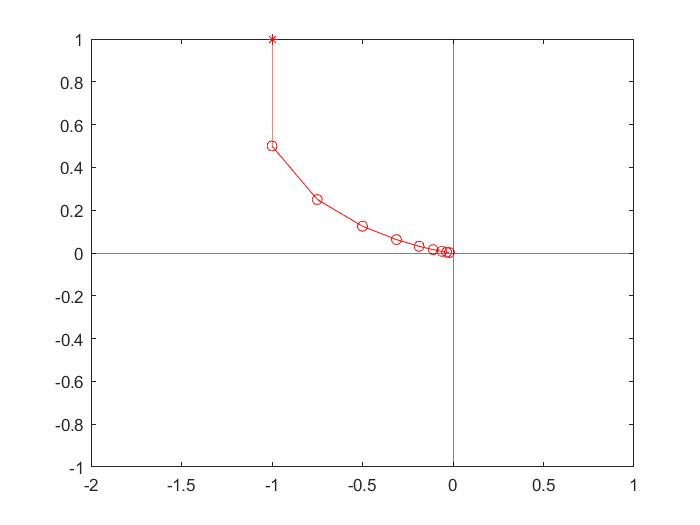
\includegraphics[width=50mm,scale=1]{Matlab3}\\
    for $\fontbf{x} = \newVec{-1}{0}$:\\
    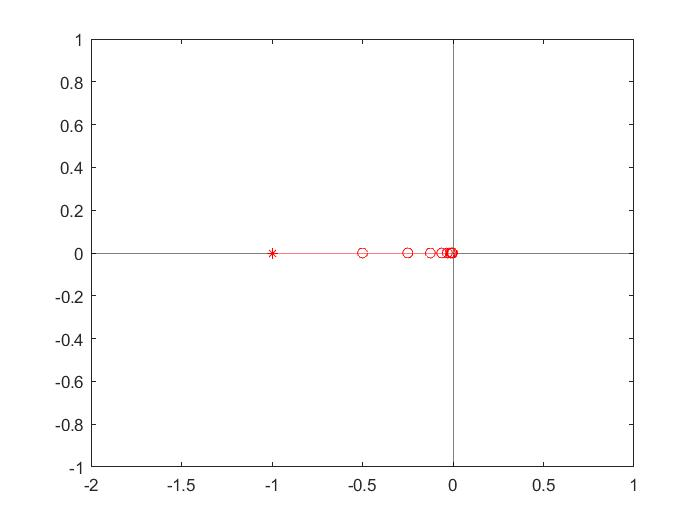
\includegraphics[width=50mm,scale=1]{Matlab4}\\\newpage
    for $\fontbf{x} = \newVec{0.5}{-1}$:\\
    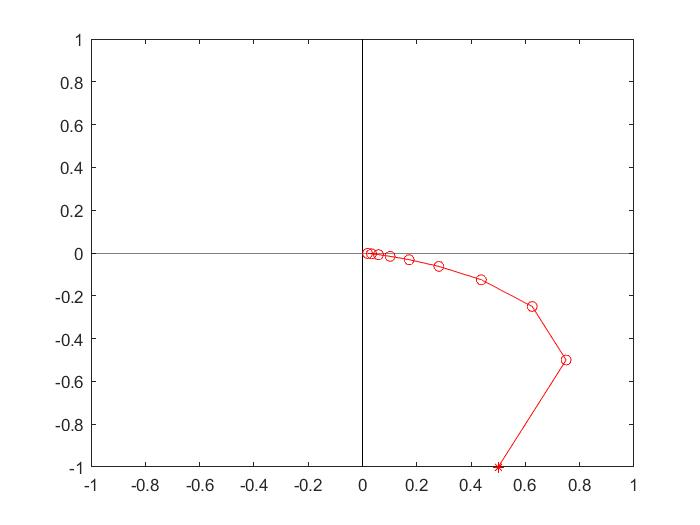
\includegraphics[width=50mm,scale=1]{Matlab5}\\
    }
    
\end{enumerate}
\item 
$A = \newtt{0}{0.5}{-0.5}{0}$
\begin{enumerate}
    \item $\textbf{x}_0 = \newVec{1}{1}\\ \textbf{x}_1 = \newVec{0.5}{-0.5}\\ \textbf{x}_2 = \newVec{-0.25}{0.25}\\ \textbf{x}_3 = \newVec{0.125}{-0.125}$\\
        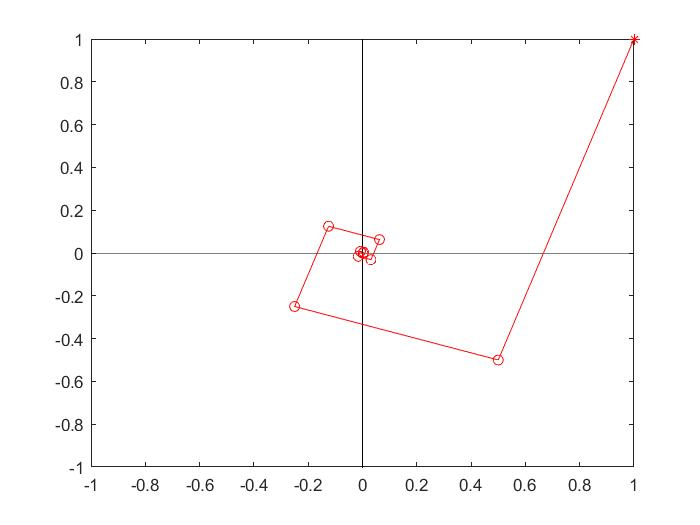
\includegraphics[width=50mm,scale=1]{Matlab1_1.jpg}
    \item $\textbf{x}_0 = \newVec{1}{0}\\ \textbf{x}_1 = \newVec{0}{-0.5}\\ \textbf{x}_2 = \newVec{-0.25}{0}\\ \textbf{x}_3 = \newVec{0}{0.125}$\\
        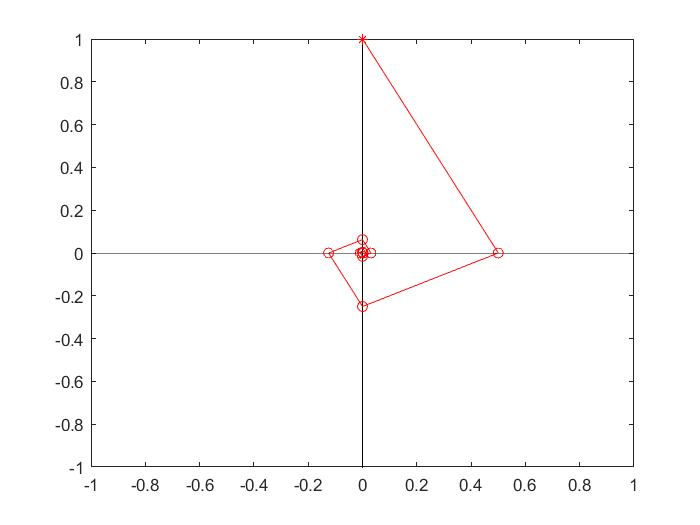
\includegraphics[width=50mm,scale=1]{Matlab1_2.jpg}
    \item $(-\lambda)^2 + 0.25 = 0\\
            \lambda = \sqrt{-0.25} = 0.5i$\\\\
            $0.5i\newVec{x}{y} = \newtt{0}{0.5}{-0.5}{0}\newVec{x}{y}$\\
            $(0.5i)x = 0.5y \rightarrow ix = y$, so the eigenvalue for $\lambda = 0.5i$ is $\newVec{1}{i}$\\
             $(-0.5i)x = 0.5y \rightarrow -ix = y$, so the eigenvalue for $\lambda = -0.5i$ is $\newVec{1}{-i}$\\
             So the general solution is $\textbf{x}_0 = C_1 (0.5i)\newVec{1}{i} + C_2 (-0.5i)\newVec{1}{-i}$, or for $\textbf{x}_k$: $\textbf{x}_k = C_1 (0.5i)^k\newVec{1}{i} + C_2 (-0.5i)^k\newVec{0}{-i}$\\
             As the $\lim_{k\to\infty} \textbf{x}^k \rightarrow \newVec{0}{0}$ for all $C_1, C_2, x_0$. So the origin is an attractor.
    \item{
    for $\fontbf{x} = \newVec{-1}{1}$:\\ 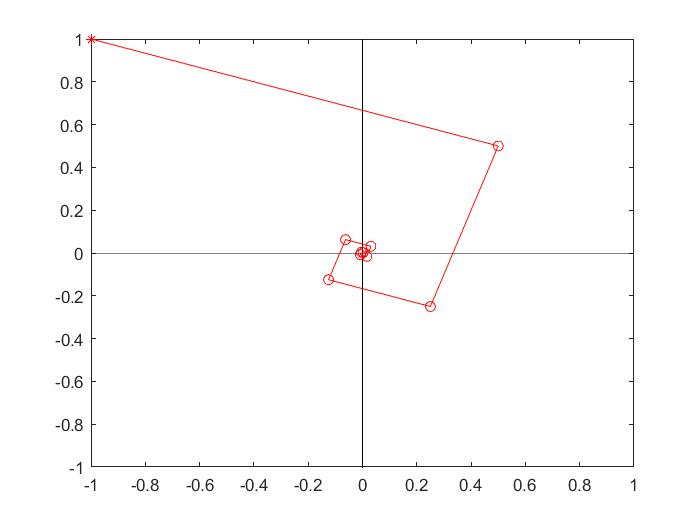
\includegraphics[width=50mm,scale=1]{Matlab1_3}\\\newpage
    for $\fontbf{x} = \newVec{-1}{0}$:\\
    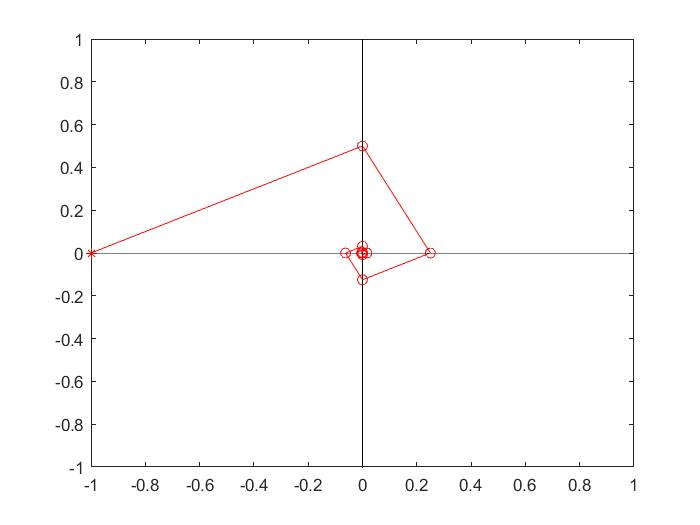
\includegraphics[width=50mm,scale=1]{Matlab1_4}\\
    for $\fontbf{x} = \newVec{0.5}{-1}$:\\
    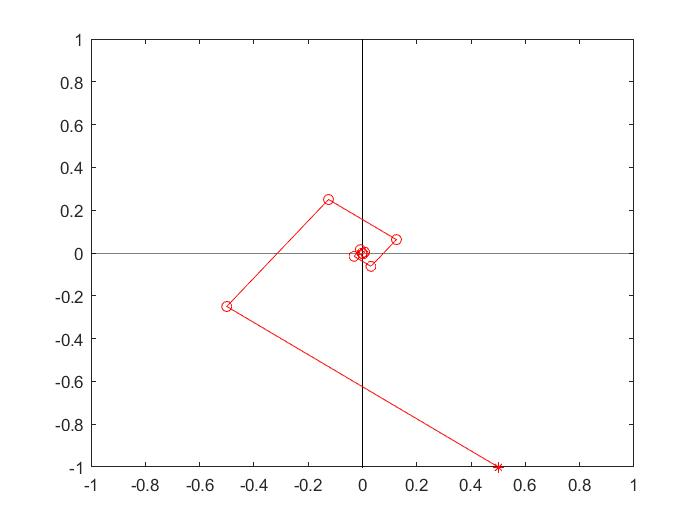
\includegraphics[width=50mm,scale=1]{Matlab1_5}\\
    }
\end{enumerate}

\newcommand{\matP}{\newttt{\frac{1}{2}}{\frac{1}{3}}{\frac{1}{3}}{0}{\frac{1}{3}}{\frac{2}{3}}{\frac{1}{2}}{\frac{1}{3}}{0}}
\newcommand{\matPmult}{\newttt{3}{2}{3}{0}{2}{4}{3}{2}{0}}
\newcommand{\newtttdet}[9]{\begin{vmatrix}#1 & #2 & #3\\ #4 & #5 & #6 \\ #7 & #8 & #9\end{vmatrix}}

\item
$P = \matP$\\
We know by theorem 4.30, if we have a Markov matrix, which we do, then there is only one positive eigenvalue, which is 1.\\\\
$\newVect{x}{y}{z} = \matP \newVect{x}{y}{z}$\\
$6\newVect{x}{y}{z} = \matPmult \newVect{x}{y}{z}$\\\\\\
Char Eq: \\
$0 = \newtttdet{-3}{2}{2}{0}{-4}{4}{3}{2}{-6} = \newtttdet{-3}{2}{2}{0}{-4}{4}{0}{4}{-4} = \newtttdet{-3}{2}{2}{0}{-4}{4}{0}{0}{0} \rightarrow \newVect{x}{y}{z} = \newVect{\frac{4}{3} z}{z}{0}$\\
So the eigenvector, and steady state vector, is $\newVect{4}{3}{0}$.

\item
$L = \newttt{1}{5}{3}{\frac{1}{3}}{0}{0}{0}{\frac{2}{3}}{0}$\\\\
We know there is one positive eigenvalue, and one positive eigenvector, by theorem 4.35.\par
Char eq: $0 = (1-\lambda)\lambda^2 - 5(\frac{-\lambda}{3}) + 3(\frac{2}{3}) = \lambda^3 - \lambda^2 - \frac{5}{3}\lambda + \frac{2}{3}$\par
The only positive solution to the above equation is: $\lambda = 2$.\\\\
Solving for the eigenvector:\\
$2\newVect{x}{y}{z} = \newttt{1}{5}{3}{\frac{1}{3}}{0}{0}{0}{\frac{2}{3}}{0} \newVect{x}{y}{z}$\\
$6\newVect{x}{y}{z} = \newttt{3}{15}{9}{1}{0}{0}{0}{2}{0}\newVect{x}{y}{z}$\\
$0 = \newttt{-3}{15}{9}{1}{-6}{0}{0}{2}{-6} \newVect{x}{y}{z}$\\
$0 = \newttt{0}{-3}{9}{1}{-6}{0}{0}{2}{-6} \newVect{x}{y}{z}$\\
$0 = \newttt{0}{0}{0}{1}{-6}{0}{0}{2}{-6} \newVect{x}{y}{z}$\\\\\\
So the eigenvector looks like: $\newVect{x}{y}{z} \rightarrow \newVect{1}{\frac{1}{6}}{\frac{1}{18}} \rightarrow \newVect{18}{3}{1}$\\\\\\
So the positive eigenpair is $(2, \newVect{18}{3}{1})$.



\end{enumerate}

\end{document}